%!TEX root = ../thesis_a4.tex

%\part{Knowledge-based Approaches}
%\label{part:knowledge-based}

\chapter[Semantic Enrichment for Similarity and Classification][Semantic Enrichment for Sim. and Classif.]{Semantic Enrichment for Similarity and Classification}
\label{sec:similarity}

\section{Introduction}\label{sec:similarity:introduction} %Todos

This chapter describes several methods for the semantic enrichment of music documents using Entity Linking and their application in the context of two widely studied MIR tasks, artist similarity and music genre classification. 
First, a method for computing semantic similarity at document-level is presented. The cornerstone of this work is the intuition that semantifying and formalizing relations between entities in documents (both at in-document and cross-document levels) can represent the relatedness of two documents. Specifically, in the task of artist similarity, this derives in a measure to quantify the degree of relatedness between two artists by looking at their biographies. The evaluation results indicate that semantic based apporaches clearly outperform a baseline based on shallow word co-occurrence metrics.
%Our experiments start with a preprocessing step which involve Entity Linking over artist biographical texts.
%Then, a knowledge representation is derived from the detected entities in the form of a semantic graph or a mapping to a vector-space model.
%Finally, different similarity measures are applied to a benchmarking dataset. The evaluation results indicate that some approaches presented in this chapter clearly outperform a baseline based on shallow word co-occurrence metrics.
%Source code and datasets are available online\footnote{\url{http://mtg.upf.edu/downloads/datasets/semantic-similarity}}.
%Second, we explore the contribution of such features to the Music Genre classification task, consisting in, given a song or album review, predict the genre it belongs to.
Second, we perform experiments on music genre classification from album customer reviews, exploring a variety of feature types, including semantic features obtained through Entity Linking, sentimental features  and acoustic features. These experiments show that modeling semantic information contributes to outperforming strong bag-of-words baselines. 

The remainder of this chapter is structured as follows: Section \ref{sec:similarity:similarity} describes a methodology for computing artist similarity from artist biographies using semantic information. Within this section, different types of knowledge representations and similarity measures are described. Then, the settings in which experiments were carried out together with the evaluation metrics used are presented. Finally, evaluation results are presented and the performance of our method discussed. Section \ref{sec:similarity:classification} describes a methodology for computing music genre classification using album customer reviews. In this section, a dataset of music reviews is first described. Then, the different types of employed features are outlined. An experiment on genre classification is performed and results are discussed. 
Finally Section \ref{sec:similarity:conclusion} summarizes the main topics covered in this chapter.

\section{Artist similarity}
\label{sec:similarity:similarity}

We propose a method for leveraging semantic information extracted from music related documents and knowledge repositories, for the computation of a similarity measure between musical entities. In this case we focus on computing similarity between artists based on their biographies. 

The proposed method can be divided in three main steps, as depicted in Fig~\ref{fig:similarity:methodology}.
The first step consists on the application of an Entity Linking process to every document. 
The second step derives a semantically motivated knowledge representation from the identified entities. This can be achieved by exploiting natural language text as anchor between entities, or by incorporating semantic information from an external Knowledge Base. In the latter case, a document is represented either as a semantic graph or as a set of semantic vectors projected on a vector space.
Finally, the third step computes a similarity measure between documents (artist biographies in our case) based on the obtained knowledge representations. %This step can take into consideration semantic similarity among entity mentions in document pairs, or the structure and content of the semantic graph.

%The following sections provide a more detailed description of each one of these steps, along with all the approaches we have considered in each step.
%A schema of the workflow we propose is shown in.

\begin{figure}[!htp]
\centerline{\framebox{
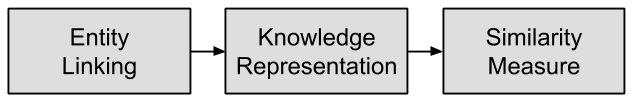
\includegraphics[width=0.75\columnwidth]{ch06_similarity_pics/methodology_bn.png}}}
\caption{Workflow of the proposed method.}
\label{fig:similarity:methodology}
\end{figure}

\subsection{Entity linking}

To obtain the entity mentions present in the documents and link them to a Knowledge Base we used Babelfy \citep{Moroetal2014b} through ELVIS (see Section~\ref{sec:linking:elvis}). Babelfy provides BabelNet URIs, and ELVIS enriches the information of every identified entity with DBpedia URIs, DBpedia Ontology types, and Wikipedia categories.
We opted to use Babelfy for consistency purposes, as in a later step we exploit \textit{SensEmbed}~\citep{Iacobaccietal2015}, a vector space representation of concepts based on BabelNet \citep{Navigli2010}. Moreover, the use of a single tool across approaches guarantees that the evaluation will only reflect the appropriateness of each one of them, and in case of error propagation all the approaches will be affected the same.

%
%Entity Linking is the task to associate, for a given candidate textual fragment, the most suitable entry in a reference Knowledge Base (KB) \cite{Moroetal2014b}. It encompasses similar subtasks such as Named Entity Disambiguation \cite{BunescuandPasca2006}, which is precisely linking mentions to entities to a KB, or Wikification \cite{MihalceaandCsomai2007}, specifically using Wikipedia as KB.

%We considered several state-of-the-art Entity Linking tools, including Babelfy \cite{Moroetal2014b}, TagMe \cite{Ferraginaetal2010}, Agdistis \cite{Usbecketal2014} and DBPedia Spotlight \cite{Mendes2011}. However we opted to use the first one for consistency purposes, as in a later step we exploit \textit{SensEmbed}~\cite{Iacobaccietal2015}, a vector space representation of concepts based on BabelNet \cite{Navigli2010}. Moreover, the use of a single tool across approaches guarantees that the evaluation will only reflect the appropriateness of each one of them, and in case of error propagation all the approaches will be affected the same.

%Babelfy \cite{Moroetal2014b} is a state-of-the-art system for Entity Linking and word sense disambiguation based on non-strict identification of candidate meanings (i.e. not necessarily exact string matching), together with a graph based algorithm that traverses the BabelNet graph and selects the most appropriate semantic interpretation for each candidate.

\subsection{Knowledge representation}\label{sec:similarity:knowledge_representations}

\subsubsection{Relations graph}\label{sec:similarity:rel_graph} %Moha

%Relation extraction has been defined as the process of identifying and annotating relevant semantic relations between entities in text \cite{JiangZhai2007}. 
In order to exploit the semantic relations between entities present in artist biographies, we applied the method defined in Chapter~\ref{sec:kb} for Relation Extraction in the music domain. The method basically consists of three steps. First, entities are identified in the text by applying Entity Linking. Second, relations between pairs of entities occurring in the same sentence are identified and filtered by analyzing the structure of the sentence, which is obtained by running a syntactic parser based on the formalism of dependency grammar~\citep{Bohnet2010}. Finally, the identified entities and relations are modeled as a knowledge graph.
%connects pairs of entities via labeled relations.
%This kind of extracted knowledge graphs may be useful for music recommendation \cite{Sordo2015}, as recommendations can be conveyed to users by means of natural language. 
We apply this methodology to the problem of artist similarity, by creating a graph that connects the entities detected in every artist biography. We call this approach RG (relations graph). Figure~\ref{fig:similarity:relation} shows the expected output of this process for a single sentence.
%Thus, two artists may be related through different paths of entities, and with different path lengths.

\begin{figure}[ht!]
    \centering
    \begin{subfigure}{\textwidth}
        \centering
        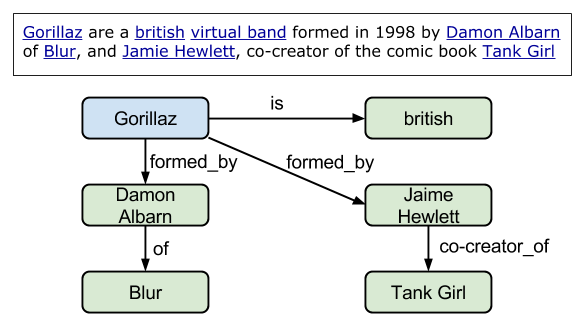
\includegraphics[width=.7\linewidth]{ch06_similarity_pics/RelationGraph.png}
    	\caption{Relation graph of a single sentence}
        \label{fig:similarity:relation}
    \end{subfigure}
    \begin{subfigure}{\textwidth}
        \centering
        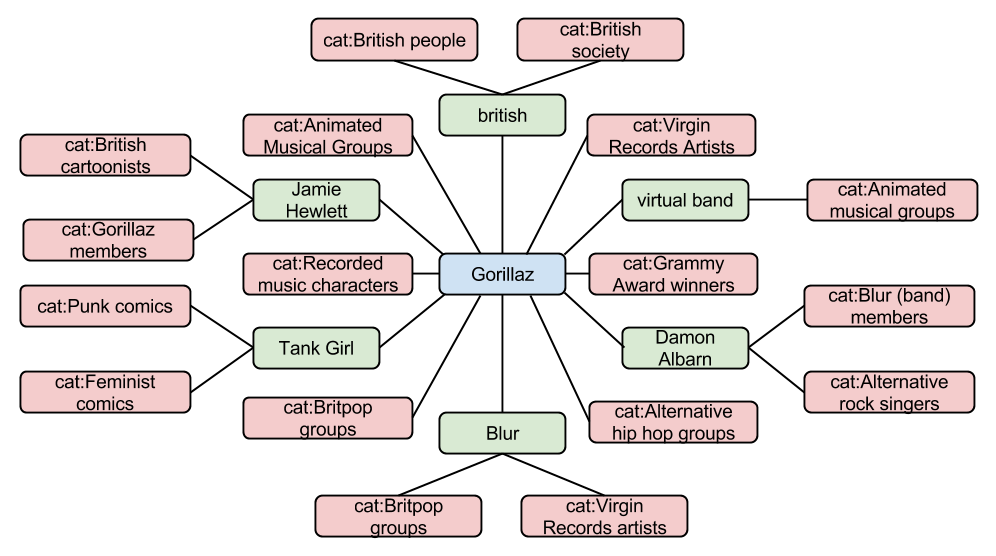
\includegraphics[width=.9\linewidth]{ch06_similarity_pics/EnrichedGraph2.png}
		\caption{Semantically enriched subgraph, variant AEC with h=2 (see MCS in Section~\ref{sec:similarity:method:sim:mcs})}
		\label{fig:similarity:enriched}
    \end{subfigure}
\end{figure}



\subsubsection{Semantically enriched graph}\label{sec:similarity:semantic_enriched_graph} %Sergio

A second approach is proposed using the same set of linked entities previously identified in the biographies. However, instead of exploiting natural language text, we use semantic information from an external Knowledge Base to enrich the semantics of the linked entities. We use semantic information coming from DBpedia. DBpedia resources are categorized using the DBpedia Ontology among others (e.g. Yago, schema.org) through the \texttt{rdfs:type} property. In addition, DBpedia resources are related to Wikipedia categories through the property \texttt{dcterms:subject}.

We take advantage of these two properties to build our semantically enriched graph.
We consider three types of nodes for this graph: 1) artist entities, obtained by matching the artist name of the biography main theme to DBPedia; 2) named entities detected by the Entity Linking step; and 3) Wikipedia categories associated to all the previous entities.
Edges are then added between artist entities and the named entities detected in their biographies, and between entities and their corresponding Wikipedia categories.
For the construction of the graph, we can select all the detected named entities, or we can filter them out according to the information related to their \texttt{rdfs:type} property. A set of six types was selected, including \textit{Artist}, \textit{Band}, \textit{Work}, \textit{Album}, \textit{MusicGenre}, and \textit{Person}, which we consider more appropriate to semantically define a musical artist.

From the previous description, we define five variants of this approach. The first variant, which we call AEC (Artists-Entities-Categories), considers all 3 types of nodes along with their relations (as depicted in Figure~\ref{fig:similarity:enriched}). The second variant, named AE (Artists-Entities) ignores the categories of the entities. The third and fourth variant, named AEC-FT and AE-FT, are similar to the first and second variant, respectively, except that the named entities are filtered using the above mentioned list of 6 entity types. Finally, the fifth variant, EC, ignores the artist entities of node type 1.


%First, artist entities are added to the graph as nodes. For every artist, all entities detected in its biography are added to the graph as nodes, and connected through an edge to the artist entity. For every added entity, its associated Wikipedia categories are retrieved and added to the graph as nodes. Every entity is attached to its associated categories though and edge. Thus, a graph of artists, linked entities and semantic categories is finally generated.
%
%A second version of the graph is proposed. Instead of adding all detected entities, we filter them out according to the information related to their \texttt{rdfs:type} property. A set of six types was selected, including \textit{artist}, \textit{band}, \textit{work}, \textit{album}, \textit{musicgenre}, and \textit{person}. These types address to the entities that we consider more appropriate to semantically define a musical artist. Hence, a filtered version of the graph is built by selecting entities only of the specified types, and their corresponding categories.
%
%For evaluation purposes, we created two more versions of the graph. Both versions follow the same graph creation process, but ignoring the last step of adding categories. Though, the graphs includes only artist entities and detected entities. One version includes all detected entities, and the other only entities of the specified types.

\subsubsection{Sense embeddings}\label{sec:similarity:sense_embeddings}

The semantic representation used in this approach is based on SensEmbed \citep{Iacobaccietal2015}. SensEmbed is a vector space semantic representation of words similar to word2vec \citep{Mikolovetal2013},
%with the aggregated value than instead of plain text words,
where each vector represents a BabelNet synset and its lexicalization. Let $A$ be the set of artist biographies in our dataset. Each artist biography $a \in A$ is converted to a set of disambiguated concepts $\text{Bfy}_{a}$ after running Babelfy over it, where each concept has a corresponding SensEmbed vector.

%where each vector represents a BabelNet synset and its lexicalization. 
%As Babelfy links entity mentions to BabelNet synsets, and every synset has a corresponding SenseEmbed vector, each artist biography $a$ is converted to a set of disambiguated concepts $\text{Bfy}_{a}$ after running Babelfy over it. 

\subsection{Similarity approaches}

\subsubsection{SimRank} %Moha

SimRank is a similarity measure based on an simple graph-theoretic model \citep{jeh2002simrank}. The intuition is that two nodes are similar if they are referenced by similar nodes. In particular we use the definition of bipartite SimRank \citep{jeh2002simrank}. We build a bipartite graph with named entities and their corresponding Wikipedia categories (the EC variant from Section~\ref{sec:similarity:semantic_enriched_graph}). The similarity between two named entities (say $p$ and $q$) is computed with the following recursive equation:

\begin{equation}
s(p,q) = \frac{C}{|O(p)||O(q)|} \sum_{i=1}^{|O(p)|} \sum_{j=1}^{|O(q)|} s(O_i(p), O_j(q))
\end{equation}

where $O$ denotes the out-neighboring nodes of a given node and $C$ is a constant between 0 and 1. For $p = q$, $s(p,q)$ is automatically set up to $1$.
Once the similarity between all pairs of entities is obtained, we proceed to calculate the similarity between pairs of artists (say $a$ and $b$) by aggregating the similarities between the named entities identified in their biographies, as shown in the following formula:

\begin{equation}
\footnotesize
sim(a,b) = Q(a,b) \frac{1}{N} \sum_{e_a \in a} \sum_{e_b \in b} s(e_a, e_b)\quad \text{if}\ s(e_a, e_b) \geq 0.1
\end{equation}

where $s$ denotes the SimRank of entities $e_a$ and $e_b$ and $N$ is the number of ($e_a$, $e_b$) pairs with $s(e_a, e_b) \geq 0.1$. This is done to filter out less similar pairs.
%We only consider pairs of entities with $s(e_a, e_b) \geq 0.1$. This is done to filter out less similar pairs.
%
Finally, $Q(a,b)$ is a normalizing factor that accounts for the pairs of artists with more similar entity pairs than others.
%, and it is computed as follows:

%\begin{equation}
%Q(a,b) = \frac{N(a,b)^{\alpha-1}}{max\_N(a)^{\alpha}}
%\end{equation}
%
%where $N(a,b)$ is the number of ($e_a$, $e_b$) pairs with $s(e_a, e_b) \geq 0.1$, and $max\_N(a)$ is the largest value of $N$ for artist $a$.
%$\alpha$ is a parameter between 0 and 1. We empirically set $\alpha = 0.6$.


\subsubsection{Maximal common subgraph}\label{sec:similarity:method:sim:mcs} %Sergio

Maximal common subgraph (MCS) is a common distance measure on graphs. It is based on the maximal common subgraph of two graphs. MCS is a symmetric distance metric, thus $d(A,B)=d(B,A)$. It takes structure as well as content into account. According to \cite{Bunke1998}, the distance between two non empty graphs $G_{1}$ and $G_{2}$ is defined as

\begin{equation}
d(G_{1},G_{2}) = 1 - \cfrac{| mcs(G_{1},G_{2}) |}{max(|G_{1}|,|G_{2}|)}
\end{equation}

It can also be seen as a similarity measure $s$, assuming that $s=1-d$, as applied in \cite{Lux2005}. To compute this similarity measure we need a graph for each artist, which may be obtained following the approaches defined in Section~\ref{sec:similarity:knowledge_representations}. An artist graph will include an artist entity node and its neighboring nodes.

Let us formally define the knowledge graph as a multi-relational graph $G=\lbrace t \mid t \in E \times R \times E \rbrace$, where $E$ denotes the set of entities and $R$ indicates the set of properties or relations, namely the edge labels. Moreover, we have $I \subseteq E$ since we consider artist items as a particular type of entities.\\
With $E^h_i$ we denote the set of entities reachable in \textit{at most h} hops from $i$ according to the shortest path in $G$. For a generic item $i$ we then define its h-hop neighborhood graph $G^h_i=\lbrace t=(e_i,r_j,e_k) \mid t \in E^h_i \times R \times E^h_i \rbrace$ that is the subgraph of $G$ induced by the set of triples involving entities in $E^h_i$. 

%Furthermore, we apply the notion of h-hop item neighborhood graph defined in \cite{ODMD14a}. Let $G=(E,P)$ be an undirected graph where $E$ represent the nodes (entities), and $P$ the set of edges with $P \subseteq E \times E$. For an artist entity $a$ in $G$, its h-hop neighborhood subgraph $G^{h}(a)=(E^{h}(a),P^{h}(a))$ is the subgraph of $G$ formed by the set of entities that are reachable from $a$ in at most h hops, according to the shortest path. %An example of a 2-hop item neighborhood graph of an artist is shown in ~Fig.
Following this approach, we obtain an h-hop item neighborhood graph for each artist. Then, maximal common subgraph is computed between the h-hop item neighborhood graphs of each pair of artists. %For each artist, the list of all similar artists ordered from the most similar to the less one is finally obtained.

\subsubsection{Cumulative cosine similarity} %Luis

%The semantic representation used in this approach is based on SensEmbed \cite{Iacobaccietal2015}, a vector space semantic representation of words similar to word2vec \cite{Mikolovetal2013}, with the aggregated value than instead of plain text words, each vector represents a BabelNet synset and its lexicalization. Specifically, the following steps are performed: (1) Let $A$ be the set of artist biographies in our dataset, in which each artist biography $a \in A$ is converted to a set of disambiguated concepts $\text{Bfy}_{a}$ after running Babelfy over it. (2)
For each pair of concepts $c \in \text{Bfy}_{a}$ and $c^{\prime} \in \text{Bfy}^{\prime}_{a}$ (as defined in Section \ref{sec:similarity:sense_embeddings}), we are interested in obtaining the similarity of their closest senses. This is achieved by first deriving the set of associated SensEmbed vectors $V_c$ and $V_{c^{\prime}}^{\prime}$ for each pair of concepts $c,\,c^{\prime}$, and then optimizing

\begin{equation}
\operatorname{max}_{v_c \in V_c , v_{c^{\prime}}^{\prime} \in V_{c^{\prime}}^{\prime}}
\left( \frac{v_c \times v_{c^{\prime}}^{\prime}}{\left\vert\left\vert{v_c}\right\vert\right\vert \left\vert\left\vert{v_{c^{\prime}}^{\prime}}\right\vert\right\vert } \right)
\end{equation}

i.e., computing cosine similarity between all possible senses (each sense represented as a vector) in an all-against-all fashion and keeping the highest scoring similarity score for each pair. Finally, the semantic similarity between two artist biographies is simply the average among all the cosine similarities between each concept pair.

\subsection{Experiments}
\label{sec:similarity:experimentalsetup}

To evaluate the accuracy of the proposed approaches we designed an experimental evaluation over two datasets. The first dataset contains 2,336 artists and it is evaluated using the list of similar artists provided by the Last.fm API as a ground truth. The second dataset contains 188 artists, and it is evaluated against user similarity judgements from the MIREX Audio Music Similarity and Retrieval task.
%More information, as well as data, can be accessed online at http://music-ir.org/mirex/wiki/MIREX\_HOME} Audio and Music Similarity evaluation dataset.
Apart from the defined approaches, a pure text-based approach for document similarity is added to act as a baseline for the obtained results.

%\subsection{Datasets}

\subsubsection{Last.fm dataset}\label{sec:similarity:lastfm_dataset}

A dataset of 2,336 artist biographies was gathered from Last.fm. The artists in this dataset share a set of restrictions.
Their biography has at least 500 characters and is written in English.
All of the artists have a correspondent Wikipedia page, and we have been able to map it automatically, obtaining the DBpedia URI of every artist.
For every artist, we queried the getSimilar method of the Last.fm API and obtained an ordered list of similar artists. Every artist in the dataset fulfills the requirement of having at least 10 similar artists within the dataset.
We used these lists of similar artists as the ground truth for our evaluation.
%As the list contains at least 10 similar artists within the dataset, we can evaluate top-10 similarity.

\subsubsection{MIREX dataset} %Moha

To build this dataset, the gathered artists from Last.fm
%(without the application of the last restriction mentioned in Section~\ref{sec:similarity:lastfm_dataset})
were mapped to the MIREX Audio Music Similarity task dataset. The AMS dataset (7,000 songs from 602 unique artists) contains human judgments of song similarity. According to~\cite{Schedl2013}, the similarity between two artists can be roughly estimated as the average similarity between their songs. We used the same approach in~\cite{Schedl2013}, that is, two artists were considered similar if the average similarity score between their songs was at least 25 (on a fine scale between 0 and 100).

%to use this dataset for artist similarity evaluation.
After the mapping, we obtained an overlap of 268 artists.
%We used this dataset of 268 artists to compute similarity using the different approaches.
As we want to evaluate Top-10 similarity, every artist in the ground truth dataset should have information of at least 10 similar artists. However, not every artist in the MIREX evaluation dataset fulfills this requirement. Therefore, after removing the artists with less than 10 similars, we obtained a final dataset of 188 artists, and used it for the evaluation.

\subsubsection{Baseline}
In order to assess the goodness of our approaches, we need a baseline approach. The baseline used in this section is a classic Vector Space Model (VSM) approach used in many Information Retrieval systems. A text document is represented as a vector of word frequencies (after removing English stopwords and words with less than 2 characters), and a matrix is formed by aggregating all the vectors. The word frequencies in the matrix are then re-weighted using \textit{tf-idf}, and finally Latent Semantic Analysis (LSA) \citep{Deerwesteretal1990} is used to produce a vector of concepts for each document. The similarity between two documents can be obtained by using a cosine similarity over their corresponding vectors.

\begin{table}[]
\small
\centering
	\begin{tabular}{  lllll }
 	\toprule
& \multicolumn{2}{c}{Precision@N} & \multicolumn{2}{c}{nDCG@N} \\
\cmidrule(lr){2-3}
\cmidrule(lr){4-5}
	Approach variants & N=5 & N=10 & N=5 & N=10 \\
	\midrule
LSA & 0.100 & 0.169 & 0.496 & 0.526 \\
RG MCS 1-hop & 0.059 & 0.087 & 0.465 & 0.476 \\
RG MCS 2-hop & 0.056 & 0.101 & 0.433 & 0.468 \\
AE MCS & 0.106 & 0.178 & 0.503  & 0.517 \\
AE-FT MCS & 0.123 & 0.183 & 0.552 & 0.562 \\
AEC MCS 1-hop & 0.120 & 0.209 & 0.573 & 0.562 \\
AEC MCS 2-hop & 0.086 & 0.160 & 0.550 & 0.539 \\
AEC-FT MCS 1-hop & \textbf{0.140} & \textbf{0.218} & \textbf{0.588} & \textbf{0.578} \\
AEC-FT MCS 2-hop & 0.100 & 0.160 & 0.527 & 0.534 \\
EC SimRank & 0.097& 0.171 &  0.509 & 0.534 \\
SE Cosine & 0.095 & 0.163 & 0.454 & 0.484 \\
\bottomrule	
	\end{tabular}
	\caption[Precision and nDCG for Top-N artist similarity in the MIREX dataset.]{Precision and normalized discounted cumulative gain for Top-N artist similarity in the MIREX dataset (N=\{5, 10\})}	
	\label{tbl:similarity:res_mirex}
\end{table}

\begin{table}
\small
\centering
	\begin{tabular}{ lllll }
 	\toprule
	& \multicolumn{2}{c}{Precision@N} & \multicolumn{2}{c}{nDCG@N} \\
\cmidrule(lr){2-3}
 \cmidrule(lr){4-5}
	Approach variants & N=5 & N=10 & N=5 & N=10 \\
	\midrule
LSA & 0.090 & 0.088 & 0.233 & 0.269 \\
RG MCS 1-hop & 0.055 & 0.083 & 0.126 & 0.149 \\
AE MCS & 0.124 & 0.200 & 0.184 & 0.216 \\
AE-FT MCS & 0.136 & 0.201 & 0.224 & 0.260 \\
AEC MCS 1-hop & 0.152 & 0.224 & 0.277 & 0.297 \\
AEC-FT MCS 1-hop & \textbf{0.160} & \textbf{0.242} & \textbf{0.288} & \textbf{0.317} \\
\bottomrule
	\end{tabular}
	\caption[Precision and nDCG for Top-N artist similarity in the Last.fm dataset.]{Precision and normalized discounted cumulative gain for Top-N artist similarity in the Last.fm dataset (N=\{5, 10\})}	
	\label{tbl:similarity:res_lastfm}
\end{table}

\subsubsection{Evaluated approaches}\label{sec:similarity:eval_approaches} %Sergio

From all possible combinations of knowledge representations, similarity measures and parameters, we selected a set of 10 different approach variants. The prefixes AEC, RG, EC, and AE refer to the graph representations (see Sections \ref{sec:similarity:rel_graph} and \ref{sec:similarity:semantic_enriched_graph}). %AEC refers to the artist entity categories graph, RG to the graph of relations extracted from text, and AE to a graph with artist entities and named entities.
SE refers to the sense embeddings approach, and LSA to the latent semantic analysis baseline approach. When these prefixes are followed by FT, it means that the entities in the graph have been filtered by type. The second term in the name refers to the similarity measure. MCS refers to maximal common subgraph, and SimRank and Cosine to SimRank and cumulative cosine similarity measures. MCS approaches are further followed by a number indicating the number of h-hops of the neighborhood subgraph.


\subsubsection{Evaluation measures}

To measure the accuracy of the artist similarity we adopt two standard performance metrics such as Precision@N, and nDCG@N (normalized discounted cumulative gain).
%We applied the metrics as defined in \cite{Steck13} for evaluating recommendation, but adapted to the problem of artist similarity.
Precision@N is computed as the number of relevant items (i.e., true positives) among the top-N items divided by $N$, when compared to a ground truth.
%A relevant item is an item in the list of $N$ similar artists suggested by the system for an artist $a$, that is also in the ground truth list of N similar artists of the same artist $a$.
%Recall@N (R@N) is computed as the ratio between the number of relevant items among the top-N items and the number items in the ground truth list.
Precision considers only the relevance of items, whilst nDCG takes into account both relevance and rank position. Denoting with  $s_{ak}$ the relevance of the item in position $k$ in the Top-N list for the artist $a$, then nDCG@N for $a$ can be defined as:
%%%%%%%%%%%%%%%%%%%%%%%%%%%
\begin{equation}\label{eq:recall}
\text{nDCG@N} = \frac{1 }{\text{IDCG@N}} \sum^N_{k=1} \frac{ 2^{ s_{ak}} -1 }{\log_2 (1+k)}
\end{equation}
%%%%%%%%%%%%%%%%%%%%%%%%%%%
where IDCG@N indicates the score obtained by an ideal or perfect Top-N ranking and acts as a normalization factor. We run our experiments for $N=5$ and $N=10$.
%In Tables~\ref{tbl:similarity:res_mirex} and~\ref{tbl:similarity:res_lastfm} average values of P@N and nDCG@N among all the evaluated artists are shown.

\subsection{Results and discussion}
\label{sec:similarity:results}

We evaluated all the approach variants described in Section~\ref{sec:similarity:eval_approaches} on the MIREX dataset, but only a subset of them on the Last.fm dataset, due to the high computational cost of some of the approaches.
%We initially worked on the MIREX dataset, as the number of artists was smaller and the computation of the algorithms was much faster. However, to ensure the credibility of the results, we applied some of the approach variants in a bigger dataset.

\begin{table}[]
\scriptsize
\centering
	\begin{tabular}{ lllllllll }
 	\toprule
& \multicolumn{8}{c}{Genres} \\
\cmidrule(lr){2-9}
	Approach variants & Blues & Country & Edance & Jazz & Metal & Rap & Rock & Overall\\
	\midrule
Ground Truth & 5.78 & 5.46 & 6.88 & 7.04 & 7.10 & 8.68 & 5.17 & 6.53\\
\midrule[.2pt]
LSA & 4.43 & 4.12 & 3.80 & 4.64 & 5.79 & 5.08 & 4.74 & 4.69\\
RG MCS 1-hop & 2.63 & 3.50 & 1.50 & 2.95 & 4.00 & 2.54 & 1.70 &  2.68\\
RG MCS 2-hop & 4.14 & 4.92 & 1.69 & 2.80 & 3.78 & 3.06 & 2.77 & 3.27\\
AE MCS & 5.52 & 5.15 & 4.36 & 7.00 & 4.34 & 5.36 & 4.46 & 5.11\\
AE-FT MCS & 5.43 & 6.12 & 4.16 & 6.20 & 6.32 & 5.36 & 3.77 & 5.26 \\
AEC MCS 1-hop & \textbf{7.22} & 5.92 & 5.24 & 7.12 & 5.48 & 6.92 & 4.86 & 6.02 \\
AEC MCS 2-hop & 4.22 & 3.69 & 4.56 & 6.20 & 4.55 & 4.64 & 4.09 & 4.54 \\
AEC-FT MCS 1-hop & 6.91 & \textbf{6.80} & \textbf{6.04} & \textbf{7.60} & \textbf{6.79} & \textbf{7.12} & \textbf{5.37} & \textbf{6.59} \\
AEC-FT MCS 2-hop & 4.09 & 4.36 & 5.56 & 6.72 & 4.39 & 4.16 & 3.77 & 4.67 \\
EC SimRank & 6.74 & 5.38 & 3.16 & 6.40 & 4.59 & 4.44 & 3.80 & 4.85 \\
SE Cosine & 3.39 & 5.50 & 5.32 & 5.16 & 4.31 & 5.36 & 4.31 & 4.75 \\
\bottomrule	
	\end{tabular}
	\caption[Average genre distribution of the top-10 similar artists using the MIREX dataset.]{Average genre distribution of the top-10 similar artists using the MIREX dataset. In other words, on average, how many of the top-10 similar artists are from the same genre as the query artist. LSA stands for Latent Semantic Analysis, RG for Relation Graph, SE for Sense Embeddings,  and AE, AEC and EC represent the semantically enriched graphs with Artists-Entities, Artist-Entities-Categories, and Entities-Categories nodes, respectively. As for the similarity approaches, MCS stands for Maximum Common Subgraph.}	
	\label{tbl:similarity:res_genre_distrib}
\end{table}


Table~\ref{tbl:similarity:res_mirex} shows the Precision@N and nDCG@N results of the evaluated approaches using the MIREX dataset, while Table~\ref{tbl:similarity:res_lastfm} shows the same results for the Last.fm dataset. We obtained very similar results in both datasets. The approach that gets best performance for every metric, dataset and value of N is the combination of the Artists-Entities-Categories graph filtered by types, with the maximal common subgraph similarity measure using a value of $h=1$ for obtaining the h-hop item neighborhood graphs.

Furthermore, given that the MIREX AMS dataset also provides genre data, we analyzed the distribution of genres in the top-10 similar artists for each artist, and averaged them by genres. The idea is that an artist's most similar artists should be from the same genre as the seed artist.
Table~\ref{tbl:similarity:res_genre_distrib} presents the results. Again, the best results are obtained with the approach that combines the Artists-Entities-Categories graph filtered by types, with the maximal common subgraph similarity measure using a value of $h=1$ for the h-hop item neighborhood graphs.

We extract some insights from these results. First, semantic approaches are able to improve pure text-based approaches. Second, using knowledge from an external Knowledge Base provides better results than exploiting the relations inside the text. Third, using a similarity measure that exploits the structure and content of a graph, such as maximal common subgraph, overcomes other similarity measures based on semantic similarity among entity mentions in document pairs.


\section{Music genre classification}\label{sec:similarity:classification}

In this section we describe a method to enrich music related documents with semantic and affective information, which are in turn exploited in a classification problem. To meassure the impact of the proposed approach, we perform an experiment on music genre classification. The experiment consists in, given an album review, predict the music genre it belongs to. Different combinations of features are explored, including semantic, sentimental, and acoustic. Experiments are performed on a subset of the Multimodal Album Reviews Dataset (MARD) described in Section~\ref{sec:musicology:mard}.
 %To this end we explore a variety of feature types, including semantic, sentimental and acoustic features. 
%First, we briefly describe the dataset used for training and testing, and then we provide a description of the features used for this task.


\subsection{Dataset description}
\label{sec:similarity:mard}

Starting from the MARD dataset, our purpose is to create a subset suitable for music genre classification, including 100 albums per genre class. We enforced these albums to be authored by different artists, and that review texts and audio descriptors of their songs are available in MARD. Then, for every album, we selected audio descriptors of the first song of each album as a representative sample of the album. From the original 16 genres, 3 of them did not have enough instances complying with these prerequisites (Reggae, Blues and Gospel). This results in a classification dataset composed of 1,300 albums, divided in 13 different genres. The review texts of each album were aggregated and then truncated around 1,000 characters (this length slightly varies from one album to another, as we wanted to keep the complete text of every individual review). We limited text length to avoid any bias towards popular albums.
%An album may have a number of reviews with different length each. For each album we randomly selected a subset of its reviews and concatenated their texts. We aimed to limit the cumulative length of the selected reviews of each album to 1000 characters approximately, without cropping any review. Finally, the average length of text by album in the classification dataset is 649 characters.


\subsection{Linguistic processing}
\label{sec:similarity:processing}

Given the set of documents, two linguistic processes are applied. First, following the work of \cite{DongSOS13,DongOS14}, we apply an aspect-based sentiment analysis technique to extract opinionated features from each document (see Section~\ref{sec:musicology:sentiment}). Second, we apply an Entity Linking process to each document. In this case, Entity Linking was performed taking advantage of TagMe \citep{Ferragina2012} and ELVIS (see Section~\ref{sec:linking:elvis}). TagMe provides for each detected entity its Wikipedia page id, whereas ELVIS enriches the obtained entities with DBpedia URIs, DBpedia Ontology types, and Wikipedia categories.
%An album may have a number of reviews with different length each. For each album we selected a subset of its reviews and concatenated their texts. We aimed to limit the cumulative length of the selected reviews of each album to 1000 characters approximately, without cropping any reviews. Finally, the average length of text by album in the classification dataset is 649 characters.

\subsection{Features}
\label{sec:similarity:features}
\subsubsection{Textual Surface Features}
We use a standard Vector Space Model (VSM) representation, where documents are represented as bag-of-words (BoW) after tokenizing and stopword removal. All words and bigrams (sequences of two words) are weighted using \textit{tf-idf}. 

\subsubsection{Semantic features}

We enrich the documents with semantic information thanks to the application of Entity Linking. Specifically, for each named entity disambiguated with TagMe, its Wikipedia ID and its associated Wikipedia categories are added at the end of the document as extra words. Wikipedia categories are hierarchically organized, so we enrich the documents by adding one level more of broader categories by querying DBpedia, using the \textit{skos:broader} property.
Then, a feature vector is obtained after applying a VSM approach with \textit{tf-idf} weighting to the semantically enriched texts.

%We enriched the initial BoW vectors with semantic information thanks to the Entity Linkingstep. The semantic feature vector of an album is conformed by a BoW model where instead of words, there are entity IDs and categories. For every entity detected by Tagme in the album texts, we added to BoW its correspondent Wikipedia ID and the Wikipedia categories associated to this entity. We applied the tfidf measure to the semantic features vector to compute a weight associated to every entity and category for each album.

\subsubsection{Sentiment features} 

Based on the aspects and associated polarity extracted with the applied aspect-based sentiment analysis technique (see Section~\ref{sec:similarity:processing}), we implement a set of sentiment features following \cite{Suero2014}:

\begin{itemize}
    \item Positive to All Emotion Ratio: fraction of all sentimental features which are identified as positive (sentiment score greater than 0). 
    %Ratio between the positive aspects and all the aspectes identified in the text. We consider an aspect as positive if it has an associated sentiment score greater than 0, and negative if it is below 0. 
    %This feature is given by:
    %\begin{equation}
    %    PosRatio = \frac{PosAspects}{PosAspectes + NegAspects}
    %\end{equation}
    \item Document Emotion Ratio: fraction of total words with sentiments attached. This feature captures the degree of affectivity of a document regardless of its polarity.
    %This feature is designed to capture the degree of affectivity (regardless of polarity) of a document. It is based on the ratio of identified aspects to all words in the document. 
    %\begin{equation}
    %    eRatio = \frac{TotalAspects}{TotalWords}
    %\end{equation}
    \item Emotion Strength: This document-level feature is computed by averaging sentiment scores over all aspects in the document.
    %Emotion Strength: This feature shows the average of the sentiment scores associated to all the identified aspects in a document
    \item F-Score\footnote{Not to be confused with the evaluation metric.}: This feature has proven to be useful for describing the contextuality/formality of language. It takes into consideration the presence of \textit{a priori} ``descriptive'' POS tags (nouns and adjectives), as opposed to ``action'' ones such as verbs or adverbs.
    
    %It is designed to capture the usage of certain informative part-of-speech categories by looking at their frequency $F$, as follows:
    %\begin{equation}
    %\begin{split}
    %    Fscore = 0.5 * ((nounF+adjF+prepF+artF) \\
%-(pronF+verbF+advF+intF) + 100)
    %\end{split}
    %\end{equation}
\end{itemize}

\subsubsection{Acoustic features}

Acoustic features are obtained from AcousticBrainz \citep{Porter2015}. They are computed using Essentia \citep{Bogdanov2013}. These encompass loudness, dynamics, spectral shape of the signal, as well as additional descriptors such as time-domain, rhythm, and tone.% For instance, rhythm descriptors refer to beat positions and BPM value, while tonal information includes chroma features, keys and scales .

%Acoustic features, obtained from MB, are computed The set of acoustic features used is provided by AcousticBrainz, which is described in \citep{Porter2015}. These features are computed using the Essentia library\footnote{\url{http://essentia.upf.edu/}}. They are divided into low-level and high-level features. Low-level features encompasses spectral, time-domain, rhythm, and tonal descriptors, whilst high-level are generated after applying data mining and machine learning techniques over low-level features. We only used in our experiments the set of low-level features, which includes features characterizing overall loudness, dynamics, and spectral shape of the signal, rhythm descriptors (including beat positions and BPM value), and tonal information (including chroma features, keys and scales).


\subsection{Baseline approaches}
\label{sec:similarity:baselines}
Two baseline systems are implemented. First, we implement the text-based approach described in \cite{Hu2005} for music review genre classification. In this work, a Na\"{i}ve Bayes classifier is trained on a collection of 1,000 review texts, and after preprocessing (tokenisation and stemming), BoW features based on document frequencies are generated.
The second baseline is computed using the AcousticBrainz framework for song classification \cite{Porter2015}. Here, genre classification is computed using  multi-class support vector machines (SVMs) with a one-vs.-one voting strategy. The classifier is trained with the set of low-level features present in AcousticBrainz. %The dataset is split 80-20\% for training and testing, and accuracy values are obtained after 5-fold cross validation. 
%The second baseline is the well known audio-based approach for genre classification described in \cite{Tzanetakis2002}. Their experiments are performed on the GTZAN dataset, consisting in 1,000 audio files categorized across 10 genres. Given that classification results using this approach are already present in AcousticBrainz, we directly computed the accuracy of these predictions in our dataset. % Al quitar la diferencia entre low y high level features arriba he quitado aqui la ref a high level features. Tampoco se lo que son, asi que si es importante habra q modificarlo.

%We used two different baseline approaches to compare the obtained results. First, we implemented the text-based approach described in \cite{Hu2006} for genre classification of music reviews. In this work, a Multinomial Naive Bayes classifier is applied to a dataset of 1,000 reviews. Review texts are tokenized and stemmized and then document frequency of word tokens is computed and used as feature weight of a bag-of-words vector. We trained and tested the apporach on our dataset of review texts.
%Second, the well known audio-based approach for genre classification described in \cite{Tzanetakis2002} is applied to our dataset. In this work, the classifier is applied to a dataset of 1000 audio files classified into 10 different genres, known as the GTZAN dataset. Given that classification results using this approach are already present in the set of high-level features of AcousticBrainz, we directly computed the accuracy of these predictions in our dataset.


\subsection{Experiments}

\begin{table}[]
\centering
\begin{tabular}{l r r r}
\hline
& BoW & BoW+SEM & BoW+SENT \\ 
\hline
Linear SVM       & \textbf{0.629}           & \textbf{0.691}               & \textbf{0.634}                \\
Ridge Classifier & 0.627                    & 0.689                        & 0.61                          \\
Random Forest    & 0.537                    & 0.6                          & 0.521                         \\ \hline
\end{tabular}
\caption{Accuracy of the different classifiers.}
\label{tbl:similarity:classifiers}
\end{table}

We tested several classifiers typically used for text classification, namely Linear SVM, Ridge Classifier and Nearest Centroid, using the implementations provided by the scikit-learn library\footnote{http://scikit-learn.org/}. Among them, Linear SVM has shown better performance when combining different feature sets (see Table~\ref{tbl:similarity:classifiers}). Therefore, we trained a Linear SVM classifier with L2 penalty over different subsets of the features described in Section \ref{sec:similarity:features}, which are combined via linear aggregation. Specifically, we combine the different feature sets into five systems, namely \textsc{BoW} (text features only), \textsc{BoW+SEM} (text and semantic features without broader categories), \textsc{BoW+SEMb} (text and semantic features with broader categories), \textsc{BoW+SENT} (text and sentiment features), and \textsc{BoW+SEM+SENT} (text, semantic, and sentiment features). In this way, we aim at understanding the extent to which sentiment and semantic features (and their interaction) may contribute to the review genre classification task. Note that this section is focused on the influence of textual features in genre classification, and classification based on acoustic features is simply used as a baseline for comparison. A proper combination of acoustic and textual features in text classification is a challenging problem and would require a deeper study, as the one provided in Chapter~\ref{sec:multi-class}.
The dataset is split 80-20\% for training and testing, and accuracy values are obtained after 5-fold cross validation. 
%As for training and test splits, we first divide the dataset, for each genre, in 80\% for training and 20\% for evaluation, and apply 5-fold cross-validation. We report average numbers across the 5 folds.

\begin{figure}
    \centering
    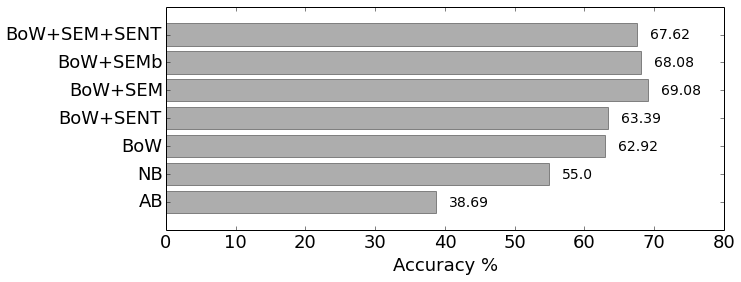
\includegraphics[width=0.7\columnwidth]{ch06_similarity_pics/results2_bn.png}
    \caption[Percentage of accuracy of the different approaches.]{Percentage of accuracy of the different approaches. AcousticBrainz refers to the AcousticBrainz framework. NB refers to the method based on Na\"{i}ve Bayes from \cite{Hu2005}.}
    \label{fig:similarity:results}
\end{figure}

%A comparison of the confusion matrix of the AcousticBrainz audio-based approach and the BoW+Sem text-based approach is shown in Table~\ref{tbl:similarity:confusion}. We observe that, although the text-based approach has higher accuracy in all the categories, both aporaches have a similar behaviour. This can explain why the combination of acoustic features with text-based features does not improve pure text-based approaches. We also note that both approaches have low accuracy values when distinguishing between Classic Rock and Alternative Rock. This means that the difference between these two categories is highly subtle, and neither acoustic nor text-based descriptors are able to properly help the classifier.


\subsection{Results and discussion}
\label{sec:similarity:class:results}

Accuracy results of the two baseline approaches introduced in Section \ref{sec:similarity:baselines} along with our approach variants are shown in Figure~\ref{fig:similarity:results}. At first sight, we may conclude that sentiment features contribute to slightly outperforming purely text-based approaches. This result implies that affective language present in a music review is not a salient feature for genre classification (at least with the technology we applied), although it certainly helps. On the contrary, semantic features clearly boost pure text-based features, achieving 69.08\% of accuracy. The inclusion of broader categories does not improve the results in the semantic approach. The combination of semantic and sentiment features improves the BoW approach, but the achieved accuracy is slightly lower than using semantic features only.%Although unreported due to space constraints, additional feature combinations were evaluated, considering for instance acoustic features, but their results were in general lower. 
% No creo que haga falta decir "lower than the systems in the figure bla", se sobreentiende no?

%Our aim in this experiment is to measure the impact of semantic and sentiment features in a text-based approach for genre classification. In addition, we want to compare these results with state-of-the-art audio-based approaches. The combination of acoustic and textual features is out of the scope of this chapter.
%The different approaches are built by linear aggregation of the different feature vectors. The approach used for genre classification is trained and tested on a Linear SVM classifier with L2 penalty. The dataset was split for each genre in 80\% for training and 20\% for testing. In addition, we applied 5-fold cross validation and averaged the results. Results of the three baseline approaches plus 3 text-based approaches with different combinations of features and are shown in Figure~\ref{fig:similarity:results}. We observe that sentiment features slightly outperforms a pure text-based approach. This result implies that measuring the positiveness or negativeness in the language used in a music review is not a salient feature for genre classification, although it certainly help. By contrast, semantic features really boost accuracy. The addition of external semantic information related to the entities present in the review help in the process of classification. We tried further combinations of features, including semantic, sentimental and acoustic features, but results did not improve the ones presented in Figure~\ref{fig:similarity:results}.

Let us review the results obtained with baseline systems. The Na\"{i}ve Bayes approach in \cite{Hu2005} is reported to achieve an accuracy of 78\%, while in our results it is below 55\%. The difference in accuracy may be due to the substantial difference in length of the review texts. In \cite{Hu2005}, review texts were at least 3,000 characters long, much larger that ours. Moreover, the addition of a distinction between Classic Rock and Alternative Rock is penalizing our results. 
As for the acoustic-based approach, although the obtained accuracy may seem low, it is in fact a good result for purely audio-based genre classification, given the high number of classes and the absence of artist bias in the dataset \citep{bogdanov2016cross}.
%As for the acoustic-based approach defined in \cite{Tzanetakis2002}, they achieve 61\% accuracy on the GZTAN dataset. However, certain bias in this dataset \cite{Sturm2012} may be responsible of such high performance. Therefore, we have taken the computation done in AcousticBrainz using this approach and trained on the GZTAN dataset to our dataset. As this approach classify a song among 10 different genres, and our dataset have 13 genres, we computed the average accuracy among the results only for this 10 genres. 
Finally, we refer to Figure~\ref{fig:similarity:confusion} to highlight the fact that the text-based approach clearly outperforms the acoustic-based classifier, although in general both show a similar behaviour across genres. Also, note the low accuracy for both Classic Rock and Alternative Rock, which suggests that their difference is subtle enough for making it a hard problem for automatic classification.

%We  did some trials at different character length, and this aspect revealed to be very determinant in the accuracy results. After performing several tests did some trials at different character length, and this aspect revealed to be very determinant in the accuracy results. In addition, the addition of a distinction between Classic and Alternative Rock is penalizing the results, as it has shown to be a difficult task. However, the aim of this experiment is compare different approaches among them, rather than achieving a very high value of accuracy.
%Furthermore, the acoustic-based approach defined in \cite{Tzanetakis2002} presents a result of 61\% of accuracy in the GZTAN dataset. However, some biases in the dataset \cite{Sturm2012} may be responsible of such a high level. Therefore, we have taken the computation done in AcousticBrainz using this approach and trained on the GZTAN dataset to our dataset. As this approach classify a song among 10 different genres, and our dataset have 13 genres, we computed the average accuracy among the results only for this 10 genres.


\begin{figure}[ht!]
    \centering
    \begin{subfigure}{.45\textwidth}
        \centering
        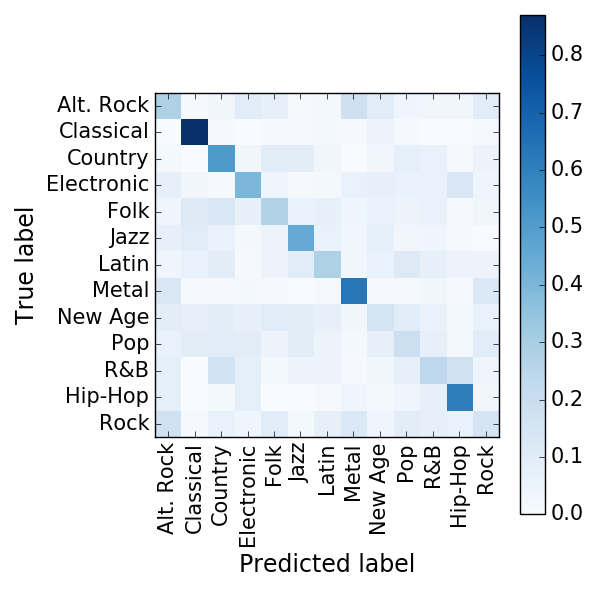
\includegraphics[width=\linewidth]{ch06_similarity_pics/confusion_audio.png}
    	\caption{AcousticBrainz acoustic-based.}
    \end{subfigure}
    \begin{subfigure}{.45\textwidth}
        \centering
        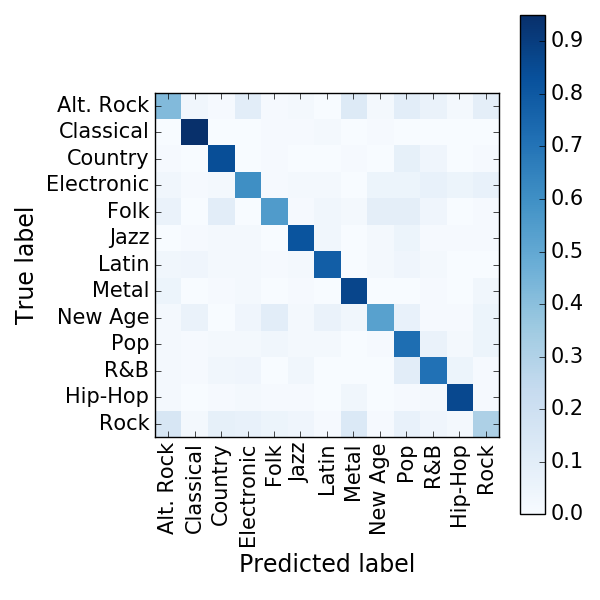
\includegraphics[width=\linewidth]{ch06_similarity_pics/confusion_text.png}
		\caption{BoW+SEM text-based.}
    \end{subfigure}
    \caption{Confusion matrix.}
	\label{fig:similarity:confusion}
\end{figure}

\section{Conclusion}
\label{sec:similarity:conclusion}

In this chapter we presented several methodologies that exploit semantic technologies for computing artist similarity and music genre classification. Particularly, we focused on the use of Entity Linking as a medium to enrich the information present in musical documents. Results in both tasks show that the addition of semantic information via Entity Linking clearly yields performance improvements.

Different methods to embed this semantic information have been proposed, from knowledge graphs to vector space models.
In the case of artist similarity, the proposed methodology is divided in three main steps: First, named entity mentions are identified in the text and linked to a Knowledge Base. Then, these entity mentions are used to construct a semantically motivated knowledge representation. Finally a similarity function is defined on top of the knowledge representation to compute the similarity between artists.
For each one of these steps we explored several approaches, and evaluated them against a small dataset of 188 artist biographies, and a larger one of 2,336, both obtained from Last.fm.
Results showed that the combination of semantically enriched graphs via Entity Linking, and a maximal common subgraph similarity measure clearly outperforms a baseline approach that exploits word co--occurrences and latent factors.

In the case of music genre classification, a multimodal dataset of album customer reviews combining text, metadata and acoustic features gathered from Amazon, MusicBrainz and AcousticBrainz respectively was used. Customer review texts were further enriched with data from Wikipedia along with polarity information derived from aspect-based sentiment analysis. Based on this information, a classifier is trained using different combinations of features. 
A comparative evaluation of features suggests that a combination of text and semantic information has higher discriminative power, outperforming competing systems in terms of accuracy.

In the light of these results on both tasks, the following conclusions can be drawn: The described semantic enrichment approaches outperform pure text-based approaches thanks to the enrichment of texts with knowledge leveraged from external ontologies. We have observed that the inclusion of this external knowledge boosts the performance on both tasks. In addition, reducing noise by filtering linked entities by type is a rewarding step that contributes to an improved performance.
